\section{Modules}
\SectionPage

\begin{frame}
  \frametitle{UI framework}
  \begin{figure}[H]
    \centering
    \begin{tikzpicture}
  \node (window) [rectangle, draw, minimum height=7cm, minimum width=10cm] at (0, 0) {};
  \node (menu) [rectangle, draw, minimum height=0.5cm, minimum width=10cm] at (0, 3.25) {Menu};
  \node (tabs) [rectangle, draw, minimum height=0.25cm, minimum width=8cm] at (1, 2.75) {Tabs};
  \node (tab) [rectangle, draw, minimum height=0.25cm, minimum width=1cm] at (-2.5, 2.75) {Tab};
  \node (sidebar) [rectangle, draw, minimum height=6.5cm, minimum width=2cm] at (-4, -0.25) {Sidebar};
  \node (content) [rectangle, draw, minimum height=6.5cm, minimum width=8cm] at (1, -0.25) {Content};
\end{tikzpicture}
    \caption{
      Diagram of the layout of different areas in our IDE
    }
    \label{fig:ideLayout}
  \end{figure}
\end{frame}

\begin{frame}
  \frametitle{File system operations (FSA)}
  Since this IDE can target different OSes, we
  need some form of FSA. This is achieved by our module, ide\_fsa, which
  enables other modules to do file system operations without having to worry about
  what OS they are on.
\end{frame}

\begin{frame}
  \frametitle{Cache}
  Cache stuff
\end{frame}

\begin{frame}
  \frametitle{Module installer}
  Module installing
\end{frame}

\begin{frame}
  \frametitle{Event sender}
  \begin{figure}
    \centering
    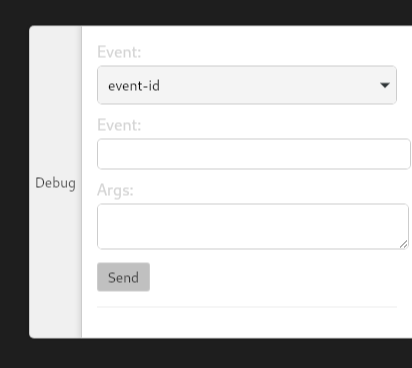
\includegraphics[width=0.5\textwidth]{./pics/event-mocking.png}
    \caption{
      Form for sending events
    }
  \end{figure}
\end{frame}

\begin{frame}
  \frametitle{State visualization}
  \begin{figure}
    \centering
    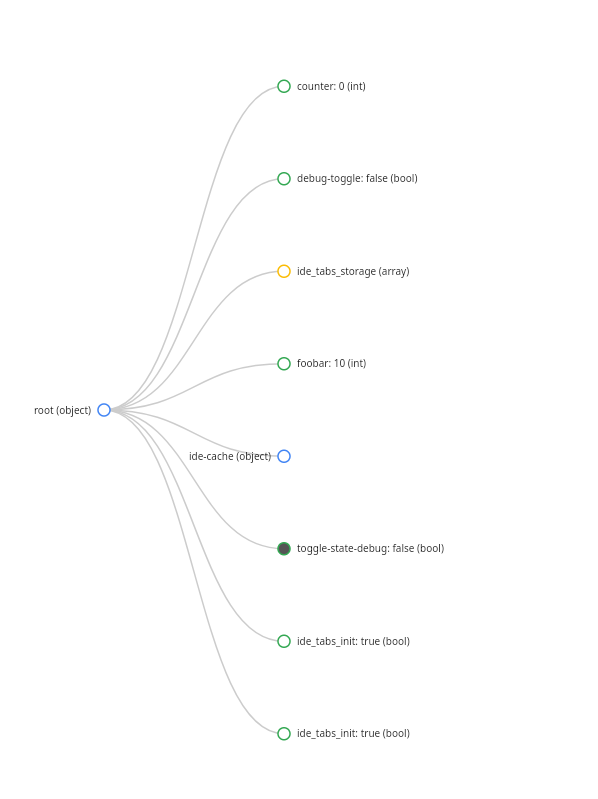
\includegraphics[width=0.5\textwidth]{./pics/debug-state.png}
    \caption{
      Visualization of the state
    }
  \end{figure}
\end{frame}

\begin{frame}
  \frametitle{Error reporting}
\end{frame}

\begin{frame}
  \frametitle{File explorer}
  \begin{figure}
    \centering
    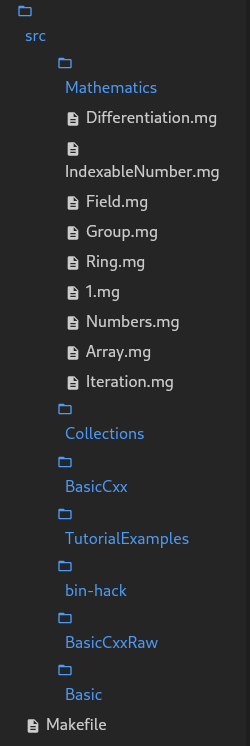
\includegraphics[width=0.5\textwidth]{./pics/ide-explorer.png}
    \caption{
      File explorer module
    }
  \end{figure}
\end{frame}

\begin{frame}
  \frametitle{File icons}
\end{frame}

\begin{frame}
  \frametitle{Tabs}
\end{frame}

\begin{frame}
  \frametitle{Editor}
\end{frame}

\begin{frame}
  \frametitle{Magnolia dependency graph}
\end{frame}

\begin{frame}
  \frametitle{Rust dependencies}
\end{frame}

%\hidelogo

\begin{frame}
  \frametitle{Module dependency viewer}
\end{frame}

\begin{frame}
  \frametitle{Module dependencies}
  \begin{figure}
    \centering
      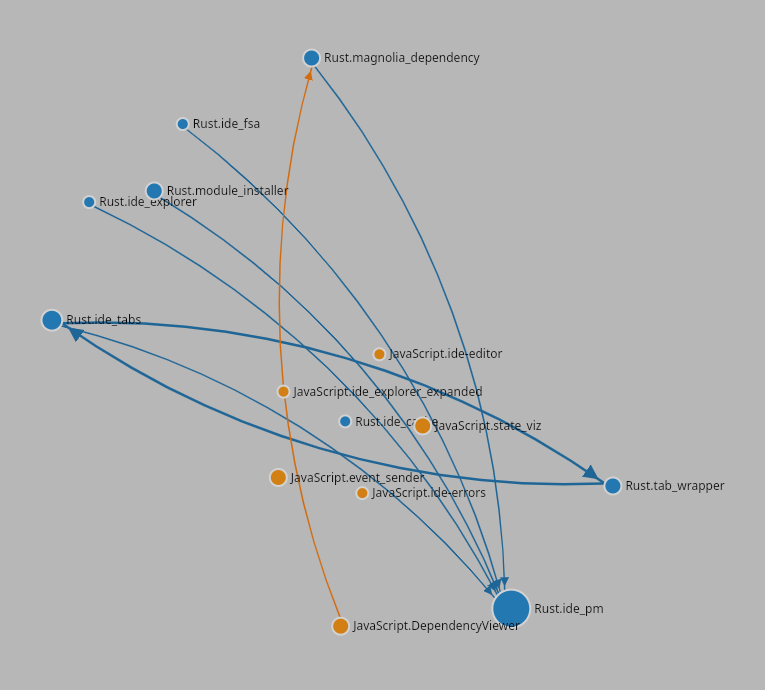
\includegraphics[width=0.7\textwidth]{./pics/module-dependencies.png}
  \end{figure}
\end{frame}

%\showlogo
